\documentclass[11pt]{article}

\usepackage[a4paper,margin=1in]{geometry}
\usepackage{amsmath,amssymb,amsthm,mathtools}
\usepackage{bm}
\usepackage{microtype}
\usepackage[hidelinks]{hyperref}
\usepackage{pgfplots}
\pgfplotsset{compat=1.18}
\hypersetup{
  pdftitle={Markovian Embeddability of SU(2)-Covariant Spin Channels},
  pdfauthor={Anonymous},
  pdfsubject={Covariant quantum Markov semigroups and channel embedding},
  pdfkeywords={SU(2), quantum channels, GKSL generators, Markovian embedding,
    Wigner 6j symbols, CP-divisibility}
}

\newtheorem{theorem}{Theorem}[section]
\newtheorem{lemma}[theorem]{Lemma}
\newtheorem{proposition}[theorem]{Proposition}
\newtheorem{corollary}[theorem]{Corollary}
\theoremstyle{definition}
\newtheorem{definition}[theorem]{Definition}

\newcommand{\SU}{\mathrm{SU}(2)}
\newcommand{\End}{\operatorname{End}}
\newcommand{\Tr}{\operatorname{Tr}}
\newcommand{\id}{\operatorname{id}}
\newcommand{\Ad}{\operatorname{Ad}}
\newcommand{\cL}{\mathcal L}
\newcommand{\cD}{\mathcal D}
\newcommand{\cE}{\mathcal E}
\newcommand{\cP}{\mathcal P}
\newcommand{\cU}{\mathcal U}
\newcommand{\Rplus}{\mathbb R_{\geq 0}}
\newcommand{\conv}{\operatorname{conv}}

\title{Markovian Embeddability of \(SU(2)\)-Covariant Spin Channels}
\author{Anonymous}
\date{}

\begin{document}
\maketitle

\begin{abstract}
For a fixed irreducible spin representation, we classify the quantum
Markov semigroups that commute with conjugation by \(SU(2)\).  Their
generators form a simplicial cone indexed by the nonzero tensor ranks.
We compute the generator eigenvalue matrix in terms of Wigner \(6j\)
symbols, give its closed inverse, and obtain logarithmic endpoint
inequalities for spins \(1\), \(3/2\), and \(2\).  The same cone
characterizes the instantaneous logarithmic derivative of the absolute
tensor-sector eigenvalues along any invertible differentiable covariant
CP-divisible path.
\end{abstract}

\section{Introduction}

The embedding problem asks what a single quantum channel reveals about
a possible continuous-time evolution: given \(\Phi\), does there exist a
GKSL generator \(\cL\) and a time \(t>0\) such that
\(\Phi=e^{t\cL}\)?  General finite-dimensional criteria must contend
with matrix logarithm branches and conditional complete positivity
\cite{WolfEisertCubittCirac2008}.  Symmetry changes that problem
substantially when it forces both the channel and the generator to be
scalar on a multiplicity-free decomposition.

For irreducible \(SU(2)\) representations, the static channel geometry
is explicit.  Al Nuwairan proved that the EPOSIC channels are precisely
the extreme points of the covariant-channel simplex
\cite[Proposition~4.1]{AlNuwairan2014}.  The same vertices appear as
Clebsch--Gordan channels in
\cite[Sec.~2]{ChangKimKwakLeeYoun2022}, where low-rank entanglement and
degradability questions are analyzed, in particular in Sec.~4.
C{\^i}rstoiu, Korzekwa, and Jennings describe the simplex in Liouville
coordinates and derive the action of its extremal channels on
irreducible tensor operators
\cite[Theorem~7 and Appendix~B]{CirstoiuKorzekwaJennings2020}.
Aschieri, Ruba, and Solovej developed quantitative large-spin
approximations and trace formulas for this simplex
\cite[Sec.~1]{AschieriRubaSolovej2024}.  Recent work on Weyl dynamical
maps gives semigroup and non-Markovianity criteria in a different
covariant family \cite[Proposition~2]{XuJagadish2026}.
Rudnicki, Klimov, Mu{\~n}oz, Leuchs, and S{\'a}nchez-Soto have also given a
recent Choi--Kraus characterization of the static \(SU(2)\)-covariant
channel family
\cite[Abstract]{RudnickiKlimovMunozLeuchsSanchezSoto2026}.

The continuous-time covariance principle predates the present
specialization.  Holevo showed that the completely positive part in a
standard representation of a norm-continuous covariant semigroup may
be chosen covariant and its Hamiltonian may be chosen to commute with
the symmetry representation \cite[Abstract]{Holevo1993}; the
form-generator theory beyond norm continuity is developed in
\cite[Abstract]{Holevo1995}.  In the finite-dimensional irreducible
spin setting, the multiplicity-free adjoint decomposition resolves
Holevo's covariant completely positive part into one scalar rate per
tensor rank.  We include that specialization with the normalization
needed for the embedding calculation.

Here the symmetry is imposed on the continuous-time generator as well
as on its endpoint.  Thus ``embeddable'' below means embeddable by an
\(SU(2)\)-covariant GKSL generator; no assertion is made about a
noncovariant logarithm of the same endpoint.  The main results are:
\begin{enumerate}
 \item every invariant generator is a unique nonnegative combination
 of the tensor-rank dissipators \(\cD_k\);
 \item its sector eigenvalue matrix \(M^{(j)}\) and the inverse matrix
 are single \(6j\)-symbol formulas;
 \item positivity of all sector eigenvalues together with
 \((M^{(j)})^{-1}\log\bm\eta\geq0\) is necessary and sufficient for
 endpoint embeddability, yielding explicit facets through spin \(2\);
 \item the same inequalities applied to
 \(d(\log|\bm\eta(t)|)/dt\) characterize all invertible differentiable
 covariant CP-divisible paths, including paths on fixed negative-spectrum
 branches.
\end{enumerate}
All low-spin matrices, intersections, and plotted meshes are generated
by exact symbolic scripts included with the paper.

\section{Tensor conventions and covariant channels}

Let \(j\in\tfrac12\mathbb N_0\), let \(\mathcal H_j\) be the spin-\(j\)
irreducible unitary representation, and put \(d=2j+1\).  Conjugation
defines the unitary representation
\[
  \cU_g(X)=U_j(g)XU_j(g)^\dagger
  \quad\text{on }B(\mathcal H_j).
\]
The Clebsch--Gordan decomposition is multiplicity free:
\begin{equation}\label{eq:adjoint-decomposition}
  B(\mathcal H_j)\cong \mathcal H_j\otimes\mathcal H_j^*
  \cong \bigoplus_{\ell=0}^{2j}V_\ell.
\end{equation}

We use the Hilbert--Schmidt orthonormal spherical tensors of
Breuer~\cite[Appendix A, Eqs.~(A1)--(A6)]{Breuer2005}.  In the angular
momentum basis they are
\begin{equation}\label{eq:tensor-definition}
 \langle j,m_1|T_q^{(k)}|j,m_2\rangle
 =\sqrt{2k+1}\,(-1)^{j-m_1}
 \begin{pmatrix}
 j&j&k\\ m_1&-m_2&-q
 \end{pmatrix}.
\end{equation}
Thus
\begin{align}
 \Tr\!\left((T_q^{(k)})^\dagger T_{q'}^{(k')}\right)
 &=\delta_{kk'}\delta_{qq'},
 &T_0^{(0)}&=I/\sqrt d,                                      \label{eq:tensor-orthogonality}\\
 \cU_g(T_q^{(k)})
 &=\sum_{r=-k}^k D^{(k)}_{rq}(g)T_r^{(k)},
 &(T_q^{(k)})^\dagger&=(-1)^qT_{-q}^{(k)}.                  \label{eq:tensor-transform}
\end{align}

\begin{lemma}[Scalar tensor sum]\label{lem:scalar-sum}
For \(0\leq k\leq 2j\),
\begin{equation}\label{eq:scalar-sum}
 \sum_{q=-k}^k (T_q^{(k)})^\dagger T_q^{(k)}
 =\sum_{q=-k}^k T_q^{(k)}(T_q^{(k)})^\dagger
 =\frac{2k+1}{d}I.
\end{equation}
\end{lemma}

\begin{proof}
The first sum is invariant under conjugation by
\eqref{eq:tensor-transform}, hence it is scalar by irreducibility of
\(U_j\).  Its trace is \(2k+1\) by
\eqref{eq:tensor-orthogonality}, which gives the first identity.  The
adjoint relation in \eqref{eq:tensor-transform} permutes the summands
of the two sums, giving the second identity.
\end{proof}

\begin{definition}[Invariant dissipators]\label{def:dissipators}
For \(1\leq k\leq2j\), define
\begin{align}
 \cD_k(X)
 &=\sum_{q=-k}^k\left(
 T_q^{(k)}X(T_q^{(k)})^\dagger
 -\frac12\{(T_q^{(k)})^\dagger T_q^{(k)},X\}\right)          \label{eq:dissipator-definition}\\
 &=\sum_{q=-k}^kT_q^{(k)}X(T_q^{(k)})^\dagger
 -\frac{2k+1}{d}X.                                           \label{eq:dissipator-simplified}
\end{align}
\end{definition}

\begin{lemma}[Dirichlet form]\label{lem:dirichlet-form}
For every \(X\in B(\mathcal H_j)\) and \(1\leq k\leq2j\),
\begin{equation}\label{eq:dirichlet-form}
 \langle X,\cD_k(X)\rangle_{\rm HS}
 =-\frac12\sum_{q=-k}^k
 \bigl\|[T_q^{(k)},X]\bigr\|_{\rm HS}^2\leq0.
\end{equation}
Consequently every entry \(M^{(j)}_{\ell k}\) introduced below is
nonpositive, and every covariantly embeddable channel satisfies
\(0<\eta_\ell\leq1\).
\end{lemma}

\begin{proof}
Write \(A_q=T_q^{(k)}\) and \(c=(2k+1)/d\).  The set
\(\{A_q\}_{q=-k}^k\) is closed under adjoints up to signs, and
Lemma~\ref{lem:scalar-sum} gives
\(\sum_qA_q^\dagger A_q=\sum_qA_qA_q^\dagger=cI\).  Expanding the
squared commutators therefore yields
\begin{equation*}
 \frac12\sum_q\|[A_q,X]\|_{\rm HS}^2
 =c\|X\|_{\rm HS}^2
 -\operatorname{Re}\sum_q\Tr(X^\dagger A_qXA_q^\dagger).
\end{equation*}
The Kraus sum is Hilbert--Schmidt self-adjoint because
\(A_q^\dagger=(-1)^qA_{-q}\), so the trace sum on the right is real.
Comparison with \eqref{eq:dissipator-simplified} proves
\eqref{eq:dirichlet-form}.  Taking \(X=T_m^{(\ell)}\) gives
\(M^{(j)}_{\ell k}\leq0\).  The final assertion follows from
\(\eta_\ell=\exp(t\sum_kM^{(j)}_{\ell k}\gamma_k)\).
\end{proof}

\begin{proposition}[Rank-one angular-momentum diffusion]
\label{prop:rank-one-diffusion}
Assume \(j>0\), and let \(J_x,J_y,J_z\) be the spin-\(j\) angular
momentum operators.  Then
\begin{equation}\label{eq:D-one-double-commutator}
 \cD_1(X)=-\frac{3}{2j(j+1)(2j+1)}
 \sum_{a=x,y,z}[J_a,[J_a,X]].
\end{equation}
In particular, its eigenvalue on \(V_\ell\) is
\begin{equation}\label{eq:M-first-column}
 M^{(j)}_{\ell1}
 =-\frac{3\ell(\ell+1)}{2j(j+1)(2j+1)}.
\end{equation}
\end{proposition}

\begin{proof}
Rotation invariance and
\(\sum_aJ_a^2=j(j+1)I\) give
\begin{equation*}
 \Tr(J_aJ_b)=s\delta_{ab},
 \qquad s=\frac{j(j+1)(2j+1)}3.
\end{equation*}
With spherical components
\(J_0=J_z\) and
\(J_{\pm1}=\mp(J_x\pm iJ_y)/\sqrt2\), the convention
\eqref{eq:tensor-definition} is \(T_q^{(1)}=J_q/\sqrt s\).
Changing unitarily from spherical to Cartesian components in
\eqref{eq:dissipator-simplified} therefore gives
\begin{equation*}
 \cD_1(X)=\frac1s\left(\sum_aJ_aXJ_a-j(j+1)X\right),
\end{equation*}
which is \eqref{eq:D-one-double-commutator}.  The adjoint Casimir
\(\sum_a[J_a,[J_a,\cdot]]\) acts on the spin-\(\ell\) summand
\(V_\ell\) by \(\ell(\ell+1)\), proving
\eqref{eq:M-first-column}.
\end{proof}

\begin{proposition}[Depolarizing direction]\label{prop:depolarizing-direction}
Let
\begin{equation}\label{eq:depolarizing-projection}
 \cP_0(X)=\frac{\Tr(X)}dI.
\end{equation}
Then
\begin{equation}\label{eq:depolarizing-generator-sum}
 \cP_0-\id=\frac1d\sum_{k=1}^{2j}\cD_k.
\end{equation}
Consequently the equal-rate point \(\gamma_k=1/d\) generates the
standard depolarizing semigroup
\begin{equation}\label{eq:depolarizing-semigroup}
 e^{t(\cP_0-\id)}(X)
 =e^{-t}X+(1-e^{-t})\frac{\Tr(X)}dI,
\end{equation}
whose nontrivial sector eigenvalues are all \(e^{-t}\).
\end{proposition}

\begin{proof}
The tensors \(T_q^{(k)}\), over all \(k,q\), form a
Hilbert--Schmidt orthonormal basis of \(B(\mathcal H_j)\).
Completeness of any such matrix basis gives
\begin{equation*}
 \sum_{k=0}^{2j}\sum_{q=-k}^k
 T_q^{(k)}X(T_q^{(k)})^\dagger=\Tr(X)I.
\end{equation*}
The \(k=0\) term is \(X/d\), and
\(\sum_{k=1}^{2j}(2k+1)=d^2-1\).  Summing
\eqref{eq:dissipator-simplified} over \(k\geq1\) therefore gives
\(\Tr(X)I-dX\), which is \eqref{eq:depolarizing-generator-sum}.
Since \(\cP_0\) is a projection and
\(\cP_0\id=\id\cP_0=\cP_0\), its exponential is
\eqref{eq:depolarizing-semigroup}.
\end{proof}

For later comparison with the complete channel simplex, set
\begin{equation}\label{eq:vertex-channel}
 \cE_k(X)=\frac{d}{2k+1}\sum_{q=-k}^k
 T_q^{(k)}X(T_q^{(k)})^\dagger,
 \qquad 0\leq k\leq2j.
\end{equation}
\begin{proposition}[Covariant-channel simplex]\label{prop:channel-simplex}
The maps \(\cE_0,\ldots,\cE_{2j}\) are precisely the vertices of the
simplex of \(\SU\)-covariant channels on \(B(\mathcal H_j)\).  Moreover,
\begin{equation}\label{eq:dissipator-vertex}
 \cD_k=\frac{2k+1}{d}(\cE_k-\id).
\end{equation}
\end{proposition}

\begin{proof}
Lemma~\ref{lem:scalar-sum} shows that every \(\cE_k\) is trace
preserving and unital.  Under column vectorization, its Choi matrix is
\(d/(2k+1)\) times the orthogonal projector onto the rank-\(k\)
summand of \(\mathcal H_j\otimes\mathcal H_j^*\).  The irreducible
Choi projectors are exactly the simplex vertices by
\cite[Sec.~1, Eqs.~(1.34)--(1.37), and Appendix A]
{AschieriRubaSolovej2024}.  Equation~\eqref{eq:dissipator-vertex}
follows by comparing \eqref{eq:dissipator-simplified} and
\eqref{eq:vertex-channel}.
\end{proof}

\section{Classification of invariant generators}

\begin{theorem}[Invariant-generator decomposition]
\label{thm:generator-classification}
A linear map \(\cL:B(\mathcal H_j)\to B(\mathcal H_j)\) generates a
norm-continuous \(\SU\)-covariant quantum Markov semigroup if and only if
there are unique numbers \(\gamma_1,\ldots,\gamma_{2j}\geq0\) such that
\begin{equation}\label{eq:generator-cone}
 \cL=\sum_{k=1}^{2j}\gamma_k\cD_k.
\end{equation}
In particular, an invariant generator has no nonzero Hamiltonian part
and is self-adjoint for the Hilbert--Schmidt inner product.
\end{theorem}

The covariance statement behind this decomposition is the
finite-dimensional compact-group case of Holevo's standard-form result
\cite[Abstract]{Holevo1993}.  The proof below identifies the unique
tensor-rank coefficients in the convention
\eqref{eq:tensor-orthogonality}.

\begin{proof}
Choose the tensors \(T_q^{(k)}\), \(1\leq k\leq2j\), as an orthonormal
basis of the traceless operators.  The canonical finite-dimensional
Gorini--Kossakowski--Sudarshan representation
\cite[Theorem~2.2 and Lemma~2.3]{GoriniKossakowskiSudarshan1976}
gives unique data
\(H=H^\dagger\), \(\Tr H=0\), and a positive semidefinite matrix \(C\)
on the traceless operator space such that
\begin{equation}\label{eq:canonical-gks}
 \cL(X)=-i[H,X]+\sum_{a,b}C_{ab}
 \left(F_aXF_b^\dagger-\frac12\{F_b^\dagger F_a,X\}\right),
\end{equation}
where \(\{F_a\}\) is the chosen tensor basis.

For \(g\in\SU\), conjugating \eqref{eq:canonical-gks} by \(\cU_g\)
replaces \(H\) by \(U_j(g)HU_j(g)^\dagger\) and \(C\) by its conjugate
under the representation of \(\SU\) on the traceless operator space.
Covariance of \(\cL\), followed by uniqueness of the canonical data,
therefore gives
\begin{equation}\label{eq:canonical-invariance}
 U_j(g)HU_j(g)^\dagger=H,
 \qquad C\cU_g=\cU_gC
 \quad(g\in\SU).
\end{equation}
Schur's lemma and irreducibility of \(U_j\) make \(H\) scalar; the
condition \(\Tr H=0\) gives \(H=0\).

By \eqref{eq:adjoint-decomposition}, the traceless operator space is
the multiplicity-free sum \(\bigoplus_{k=1}^{2j}V_k\).  A second
application of Schur's lemma gives
\begin{equation}\label{eq:gks-blocks}
 C=\bigoplus_{k=1}^{2j}\gamma_k I_{V_k}.
\end{equation}
Positivity of \(C\) is equivalent to \(\gamma_k\geq0\) for every \(k\).
Substitution of \eqref{eq:gks-blocks} into
\eqref{eq:canonical-gks} gives \eqref{eq:generator-cone}.

Conversely, each \(\cD_k\) is in GKSL form and is covariant by
\eqref{eq:tensor-transform}.  Hence every nonnegative combination in
\eqref{eq:generator-cone} generates a covariant quantum Markov
semigroup.  Uniqueness of the canonical GKS matrix gives uniqueness of
the coefficients.  Finally, the adjoint relation in
\eqref{eq:tensor-transform} shows that the Kraus sum in
\eqref{eq:dissipator-simplified} is Hilbert--Schmidt self-adjoint.
\end{proof}

\section{The exact \texorpdfstring{\(6j\)}{6j}-symbol matrix}

\begin{lemma}[Sector diagonalization and reality]
\label{lem:sector-diagonalization}
If \(A:B(\mathcal H_j)\to B(\mathcal H_j)\) is covariant, then there
are scalars \(a_0,\ldots,a_{2j}\) such that
\begin{equation}\label{eq:sector-diagonalization}
 A(T_m^{(\ell)})=a_\ell T_m^{(\ell)}
 \quad(-\ell\leq m\leq\ell).
\end{equation}
If \(A\) is Hermiticity preserving, every \(a_\ell\) is real.  If
\(A\) is a channel, then \(a_0=1\).
\end{lemma}

\begin{proof}
The irreducible summands in \eqref{eq:adjoint-decomposition} are
pairwise inequivalent and occur with multiplicity one, so
\eqref{eq:sector-diagonalization} follows from Schur's lemma.  Since
\((T_0^{(\ell)})^\dagger=T_0^{(\ell)}\), Hermiticity preservation
forces
\(a_\ell T_0^{(\ell)}=\overline{a_\ell}T_0^{(\ell)}\), hence
\(a_\ell\in\mathbb R\).  Finally, covariance makes \(A(I)\) invariant
under \(U_j\), so \(A(I)=cI\); trace preservation gives \(c=1\).
\end{proof}

For a covariant generator, write
\(\cL(T_m^{(\ell)})=\lambda_\ell T_m^{(\ell)}\).

\begin{lemma}[Tensor recoupling]\label{lem:tensor-recoupling}
For \(0\leq k,\ell\leq2j\),
\begin{equation}\label{eq:kraus-recoupling}
 \sum_{q=-k}^kT_q^{(k)}T_m^{(\ell)}(T_q^{(k)})^\dagger
 =a_{\ell k}T_m^{(\ell)},
\end{equation}
where
\begin{equation}\label{eq:a-lk}
 a_{\ell k}=(2k+1)(-1)^{2j+k+\ell}
 \begin{Bmatrix}
 j&j&k\\ j&j&\ell
 \end{Bmatrix}.
\end{equation}
\end{lemma}

\begin{proof}
The left side of \eqref{eq:kraus-recoupling} defines a covariant map,
so it is scalar on \(V_\ell\).  We calculate the scalar with the
invariant unitary
\begin{equation}\label{eq:dual-intertwiner}
 \beta:\mathcal H_j^*\longrightarrow\mathcal H_j,\qquad
 \beta\langle j,m|=(-1)^{j-m}|j,-m\rangle .
\end{equation}
For column vectorization into
\(\mathcal H_j\otimes\mathcal H_j^*\), the Kraus map in
\eqref{eq:kraus-recoupling} is represented by
\(\sum_qT_q^{(k)}\otimes\overline{T_q^{(k)}}\).  The tensors are real,
and Breuer's Eq.~(A6) states
\(\beta(T_q^{(k)})^{\mathsf T}\beta^\dagger=(-1)^kT_q^{(k)}\).
Taking adjoints gives
\begin{equation}\label{eq:dual-tensor-phase}
 \beta\,\overline{T_q^{(k)}}\,\beta^\dagger
 =(-1)^k(T_q^{(k)})^\dagger .
\end{equation}
Consequently, after applying \(I\otimes\beta\), the transfer matrix of
the Kraus map is \((-1)^kQ_k\), where
\begin{equation*}
 Q_k=\sum_{q=-k}^kT_q^{(k)}\otimes(T_q^{(k)})^\dagger
\end{equation*}
is exactly Breuer's invariant tensor
\cite[Eq.~(2.7)]{Breuer2005}.  Let \(P_\ell\) be the projector onto
the coupled spin-\(\ell\) summand.  It follows that
\begin{equation}\label{eq:a-from-QP}
 a_{\ell k}=(-1)^k\frac{\Tr(Q_kP_\ell)}{2\ell+1}.
\end{equation}
Breuer's Eqs.~(2.13)--(2.14), with \(K=k\), \(J=\ell\), and
\(j_1=j_2=j\), state
\begin{align}
 \Tr(Q_kP_\ell)
 &=\sqrt{(2k+1)(2\ell+1)}\,L_{k\ell},                       \label{eq:breuer-trace}\\
 L_{k\ell}
 &=\sqrt{(2k+1)(2\ell+1)}(-1)^{2j+\ell}
 \begin{Bmatrix}j&j&\ell\\j&j&k\end{Bmatrix}.              \label{eq:breuer-recoupling-specialized}
\end{align}
Substitution in \eqref{eq:a-from-QP}, followed by the tetrahedral
symmetry of the \(6j\) symbol, gives \eqref{eq:a-lk}.
\end{proof}

\begin{corollary}[Channel-vertex eigenvalues]\label{cor:vertex-eigenvalues}
The simplex vertex \(\cE_k\) has tensor-sector eigenvalues
\begin{equation}\label{eq:vertex-eigenvalues}
 v^{(j)}_{\ell k}
 =(2j+1)(-1)^{2j+k+\ell}
 \begin{Bmatrix}j&j&k\\j&j&\ell\end{Bmatrix},
 \qquad 0\leq k,\ell\leq2j.
\end{equation}
In particular, \(v^{(j)}_{0k}=v^{(j)}_{\ell0}=1\).
\end{corollary}

\begin{proof}
Multiply \eqref{eq:a-lk} by the normalization \(d/(2k+1)\) in
\eqref{eq:vertex-channel}.  The cases \(k=0\) and \(\ell=0\) also
follow directly from \(\cE_0=\id\) and trace preservation.
\end{proof}

\begin{theorem}[Generator eigenvalue matrix and inverse]
\label{thm:eigenmatrix}
For \(1\leq\ell,k\leq2j\), set
\begin{equation}\label{eq:M-definition}
 M^{(j)}_{\ell k}
 =(2k+1)\left[(-1)^{2j+k+\ell}
 \begin{Bmatrix}j&j&k\\j&j&\ell\end{Bmatrix}
 -\frac1{2j+1}\right].
\end{equation}
If \(\cL=\sum_k\gamma_k\cD_k\), then
\begin{equation}\label{eq:lambda-M-gamma}
 (\lambda_1,\ldots,\lambda_{2j})^{\mathsf T}
 =M^{(j)}(\gamma_1,\ldots,\gamma_{2j})^{\mathsf T}.
\end{equation}
The matrix is invertible, with
\begin{equation}\label{eq:M-inverse-formula}
 \bigl((M^{(j)})^{-1}\bigr)_{k\ell}
 =(2\ell+1)(-1)^{2j+k+\ell}
 \begin{Bmatrix}j&j&k\\j&j&\ell\end{Bmatrix}.
\end{equation}
Moreover,
\begin{equation}\label{eq:M-determinant-magnitude}
 \bigl|\det M^{(j)}\bigr|=2j+1.
\end{equation}
\end{theorem}

\begin{proof}
Equations \eqref{eq:dissipator-simplified} and
\eqref{eq:a-lk} give \eqref{eq:M-definition} and
\eqref{eq:lambda-M-gamma}.  It remains to invert the matrix.

Put \(n=2j\), \(w_r=2r+1\), and let
\(V=(v^{(j)}_{\ell k})_{0\leq\ell,k\leq n}\) be the full vertex
eigenvalue matrix from Corollary~\ref{cor:vertex-eigenvalues}.  Let
\(W=\operatorname{diag}(w_0,\ldots,w_n)\) and
\(S=\operatorname{diag}((-1)^0,\ldots,(-1)^n)\).  Breuer's
recoupling matrix is
\begin{equation*}
 L_{k\ell}=\sqrt{w_kw_\ell}\,(-1)^{n+\ell}
 \begin{Bmatrix}j&j&\ell\\j&j&k\end{Bmatrix};
\end{equation*}
it is orthogonal by the sum rule following
\cite[Eq.~(2.14)]{Breuer2005}.  Tetrahedral symmetry and
\eqref{eq:vertex-eigenvalues} give
\begin{equation}\label{eq:V-factorization}
 V=(n+1)W^{-1/2}L^{\mathsf T}W^{-1/2}S,
 \qquad
 V^{-1}=\frac1{n+1}SW^{1/2}LW^{1/2}.
\end{equation}
Hence
\begin{equation}\label{eq:V-inverse-entry}
 (V^{-1})_{k\ell}
 =\frac{w_kw_\ell}{n+1}(-1)^{n+k+\ell}
 \begin{Bmatrix}j&j&k\\j&j&\ell\end{Bmatrix}.
\end{equation}

Since the first row and first column of \(V\) consist of ones,
subtracting its first row from all other rows gives the block matrix
\begin{equation*}
 \begin{pmatrix}1&\bm 1^{\mathsf T}\\0&B\end{pmatrix},
 \qquad B_{\ell k}=v^{(j)}_{\ell k}-1
 \quad(1\leq\ell,k\leq n).
\end{equation*}
The lower-right block of \(V^{-1}\) is therefore \(B^{-1}\), while
\eqref{eq:dissipator-vertex} says
\(M^{(j)}=B\operatorname{diag}(w_1/d,\ldots,w_n/d)\).
Combining this identity with \eqref{eq:V-inverse-entry} proves
\eqref{eq:M-inverse-formula}.

Finally, \eqref{eq:V-factorization} gives
\begin{equation*}
 |\det V|=\frac{d^d}{\prod_{r=0}^nw_r}.
\end{equation*}
Row subtraction shows \(\det V=\det B\), and multiplying the
columns of \(B\) by \(w_k/d\), \(1\leq k\leq n\), gives
\(|\det M^{(j)}|=d\), proving \eqref{eq:M-determinant-magnitude}.
\end{proof}

\begin{corollary}[Dissipator--vertex conversion]
\label{cor:dissipator-vertex-conversion}
The vertex and generator eigenmatrices satisfy
\begin{equation}\label{eq:M-from-vertices}
 M^{(j)}_{\ell k}=\frac{2k+1}{2j+1}(v^{(j)}_{\ell k}-1).
\end{equation}
\end{corollary}

\begin{proof}
Restrict \eqref{eq:dissipator-vertex} to \(V_\ell\).
\end{proof}

\begin{corollary}[Complete-positivity halfspaces]
\label{cor:cp-halfspaces}
Let \(A\) be a covariant, Hermiticity-preserving, trace-preserving
map with sector eigenvalues
\(\eta_0=1,\eta_1,\ldots,\eta_{2j}\).  Define
\begin{equation}\label{eq:barycentric-weights}
 p_k=\frac{2k+1}{2j+1}
 \sum_{\ell=0}^{2j}(2\ell+1)(-1)^{2j+k+\ell}
 \begin{Bmatrix}j&j&k\\j&j&\ell\end{Bmatrix}\eta_\ell,
 \qquad 0\leq k\leq2j.
\end{equation}
Then \(A\) is completely positive if and only if \(p_k\geq0\) for
every \(k\).  In that case \(\sum_kp_k=1\) and
\begin{equation}\label{eq:channel-barycentric-decomposition}
 A=\sum_{k=0}^{2j}p_k\cE_k.
\end{equation}
\end{corollary}

\begin{proof}
In sector coordinates,
\(\bm\eta=V\bm p\), where \(V\) is the full vertex matrix used in
\eqref{eq:V-factorization}.  Formula \eqref{eq:V-inverse-entry} says
that \(\bm p=V^{-1}\bm\eta\) is exactly
\eqref{eq:barycentric-weights}.  Proposition~\ref{prop:channel-simplex}
identifies complete positivity with nonnegative barycentric weights.
The equality \(\sum_kp_k=\eta_0=1\) follows from the first row of
\(V\).
\end{proof}

\section{Endpoint embeddability}

\begin{theorem}[Covariant Markovian embedding criterion]
\label{thm:endpoint-criterion}
Let \(\Phi\) be an \(\SU\)-covariant channel on \(B(\mathcal H_j)\),
with tensor-sector eigenvalues \(\eta_0=1,\eta_1,\ldots,\eta_{2j}\).
There are \(t>0\) and an \(\SU\)-covariant GKSL generator \(\cL\) such
that \(\Phi=e^{t\cL}\) if and only if
\begin{equation}\label{eq:endpoint-criterion}
 \eta_\ell>0\quad(1\leq\ell\leq2j),
 \qquad
 (M^{(j)})^{-1}
 \begin{pmatrix}\log\eta_1\\ \vdots\\ \log\eta_{2j}\end{pmatrix}
 \in\Rplus^{2j}.
\end{equation}
\end{theorem}

\begin{proof}
If \(\Phi=e^{t\cL}\), Theorem~\ref{thm:generator-classification}
gives \(\cL=\sum_k\gamma_k\cD_k\) with \(\gamma_k\geq0\).  Its sector
eigenvalues are real by Theorem~\ref{thm:eigenmatrix}, hence
\(\eta_\ell=e^{t\lambda_\ell}>0\), and
\begin{equation*}
 \log\bm\eta=M^{(j)}(t\bm\gamma).
\end{equation*}
This proves necessity.  Conversely, define
\(r=(M^{(j)})^{-1}\log\bm\eta\geq0\) and
\(\cL=\sum_kr_k\cD_k\).  Theorem~\ref{thm:generator-classification}
makes \(\cL\) a covariant GKSL generator.  The maps \(e^{\cL}\) and
\(\Phi\) have the same scalar on every summand in
\eqref{eq:adjoint-decomposition}; therefore they are equal.
\end{proof}

\begin{corollary}[General facets and multiplicative geometry]
\label{cor:general-facets}
For a covariant channel with positive sector eigenvalues, define
\begin{equation}\label{eq:general-integrated-rates}
 r_k=\sum_{\ell=1}^{2j}(2\ell+1)(-1)^{2j+k+\ell}
 \begin{Bmatrix}j&j&k\\j&j&\ell\end{Bmatrix}\log\eta_\ell,
 \qquad 1\leq k\leq2j.
\end{equation}
Then the channel is covariantly embeddable if and only if the
\(2j\) inequalities \(r_k\geq0\) hold.  The vector \(r\) is the
unique integrated-rate vector, and the facet \(r_k=0\) is the image
of the generator face on which the rank-\(k\) dissipator is absent.

The embeddable eigenvalue set is closed under componentwise
multiplication and under weighted geometric interpolation: if
\(\bm\eta\) and \(\bm\zeta\) are embeddable and \(0\leq s\leq1\),
then so are
\begin{equation}\label{eq:multiplicative-geometry}
 \bm\eta\bm\zeta
 \quad\text{and}\quad
 \bm\eta^{\,s}\bm\zeta^{\,1-s},
\end{equation}
where all operations are componentwise.
\end{corollary}

\begin{proof}
Equation~\eqref{eq:general-integrated-rates} is
\((M^{(j)})^{-1}\log\bm\eta\) written using
\eqref{eq:M-inverse-formula}, so the first assertion is
Theorem~\ref{thm:endpoint-criterion}.  In logarithmic coordinates,
the two operations in \eqref{eq:multiplicative-geometry} add the
integrated rates and take their convex combinations, respectively.
Both preserve \(\Rplus^{2j}\).  Equivalently, all invariant generators
commute because they are diagonal on the tensor-rank sectors, so the
corresponding exponentials compose by addition of their rates.
\end{proof}

\begin{proposition}[Poisson collision representation]
\label{prop:poisson-collision}
For \(r_k\geq0\), put \(a_k=(2k+1)r_k/d\).  The semigroup endpoint
with integrated rates \(r=(r_1,\ldots,r_{2j})\) factors as
\begin{equation}\label{eq:poisson-factorization}
 \exp\left(\sum_{k=1}^{2j}r_k\cD_k\right)
 =\prod_{k=1}^{2j}
 \left[
 e^{-a_k}\sum_{m=0}^{\infty}\frac{a_k^m}{m!}\cE_k^m
 \right].
\end{equation}
Thus each extreme generator ray is the continuous-time Poissonization
of repeated applications of one Clebsch--Gordan vertex channel, and a
general invariant semigroup is the product of these commuting
processes.
\end{proposition}

\begin{proof}
Sector diagonalization makes the maps \(\cD_k\) commute.  Equation
\eqref{eq:dissipator-vertex} gives
\begin{equation*}
 e^{r_k\cD_k}
 =e^{a_k(\cE_k-\id)}
 =e^{-a_k}\sum_{m=0}^\infty\frac{a_k^m}{m!}\cE_k^m.
\end{equation*}
The series converges in operator norm.  Multiplying these identities
and using commutativity proves \eqref{eq:poisson-factorization}.
\end{proof}

\begin{corollary}[Spin \(1/2\) baseline]\label{cor:spin-one-half}
For \(j=1/2\), the covariant-channel interval is
\(-1/3\leq\eta_1\leq1\), while
\begin{equation}\label{eq:spin-one-half-criterion}
 M^{(1/2)}=(-2),\qquad
 r_1=-\frac12\log\eta_1.
\end{equation}
Consequently a spin-\(1/2\) covariant channel is covariantly
embeddable if and only if \(0<\eta_1\leq1\).  Thus every
positive-spectrum channel in this one-dimensional simplex is
embeddable.
\end{corollary}

\begin{proof}
The two channel vertices have eigenvalues \(1\) and \(-1/3\), by
\eqref{eq:vertex-eigenvalues}.  Equation~\eqref{eq:M-definition}
gives \(M^{(1/2)}=-2\), and Theorem~\ref{thm:endpoint-criterion}
gives \eqref{eq:spin-one-half-criterion}.
\end{proof}

\begin{corollary}[Spin \(1\)]\label{cor:spin-one}
For \(j=1\),
\begin{equation}\label{eq:M-spin-one}
 M^{(1)}=
 \begin{pmatrix}
 -\tfrac12&-\tfrac52\\
 -\tfrac32&-\tfrac32
 \end{pmatrix},
 \qquad
 (M^{(1)})^{-1}=
 \begin{pmatrix}
 \tfrac12&-\tfrac56\\
 -\tfrac12&\tfrac16
 \end{pmatrix}.
\end{equation}
Writing \(x_\ell=\log\eta_\ell\), a covariant channel is covariantly
embeddable if and only if \(\eta_1,\eta_2>0\) and
\begin{equation}\label{eq:spin-one-facets}
 3x_1-5x_2\geq0,
 \qquad -3x_1+x_2\geq0.
\end{equation}
Equivalently,
\begin{equation}\label{eq:spin-one-multiplicative}
 \eta_1^3\geq\eta_2^5,
 \qquad \eta_2\geq\eta_1^3.
\end{equation}
\end{corollary}

\begin{proof}
Substitution of the four relevant \(6j\) symbols into
\eqref{eq:M-definition} gives \eqref{eq:M-spin-one}.  The two rows of
its inverse, after multiplication by the positive denominator \(6\),
give \eqref{eq:spin-one-facets}.  Exponentiation gives
\eqref{eq:spin-one-multiplicative}.
\end{proof}

\begin{corollary}[Spin \(3/2\)]\label{cor:spin-three-halves}
For \(j=3/2\),
\begin{equation}\label{eq:M-spin-three-halves}
 M^{(3/2)}=
 \begin{pmatrix}
 -\tfrac15&-1&-\tfrac{14}5\\
 -\tfrac35&-2&-\tfrac75\\
 -\tfrac65&-1&-\tfrac95
 \end{pmatrix}
\end{equation}
and
\begin{equation}\label{eq:Minv-spin-three-halves}
 (M^{(3/2)})^{-1}=\frac1{20}
 \begin{pmatrix}
 11&5&-21\\
 3&-15&7\\
 -9&5&-1
 \end{pmatrix}.
\end{equation}
Writing \(x_\ell=\log\eta_\ell\), a covariant channel is covariantly
embeddable if and only if every \(\eta_\ell>0\) and
\begin{align}
 11x_1+5x_2-21x_3&\geq0,                                      \label{eq:spin-three-halves-facet-one}\\
 3x_1-15x_2+7x_3&\geq0,                                      \label{eq:spin-three-halves-facet-two}\\
 -9x_1+5x_2-x_3&\geq0.                                      \label{eq:spin-three-halves-facet-three}
\end{align}
Equivalently,
\begin{equation}\label{eq:spin-three-halves-multiplicative}
 \eta_1^{11}\eta_2^5\geq\eta_3^{21},\qquad
 \eta_1^3\eta_3^7\geq\eta_2^{15},\qquad
 \eta_2^5\geq\eta_1^9\eta_3.
\end{equation}
\end{corollary}

\begin{proof}
Substitution in \eqref{eq:M-definition} gives
\eqref{eq:M-spin-three-halves}; exact matrix inversion gives
\eqref{eq:Minv-spin-three-halves}.  The rows of the inverse give the
three inequalities, and exponentiation gives
\eqref{eq:spin-three-halves-multiplicative}.
\end{proof}

\begin{corollary}[Spin \(2\)]\label{cor:spin-two}
For \(j=2\),
\begin{equation}\label{eq:M-spin-two}
 M^{(2)}=
 \begin{pmatrix}
 -\tfrac1{10}&-\tfrac12&-\tfrac75&-3\\
 -\tfrac3{10}&-\tfrac{17}{14}&-\tfrac{11}5&-\tfrac97\\
 -\tfrac35&-\tfrac{11}7&-\tfrac9{10}&-\tfrac{27}{14}\\
 -1&-\tfrac57&-\tfrac32&-\tfrac{25}{14}
 \end{pmatrix}
\end{equation}
and
\begin{equation}\label{eq:Minv-spin-two}
 (M^{(2)})^{-1}=
 \begin{pmatrix}
 \tfrac12&\tfrac12&0&-\tfrac65\\
 \tfrac3{10}&-\tfrac3{14}&-\tfrac45&\tfrac{18}{35}\\
 0&-\tfrac47&\tfrac12&-\tfrac9{70}\\
 -\tfrac25&\tfrac27&-\tfrac1{10}&\tfrac1{70}
 \end{pmatrix}.
\end{equation}
Writing \(x_\ell=\log\eta_\ell\), a covariant channel is
covariantly embeddable if and only if every \(\eta_\ell>0\) and
\begin{align}
 5x_1+5x_2-12x_4&\geq0,                                    \label{eq:spin-two-facet-one}\\
 21x_1-15x_2-56x_3+36x_4&\geq0,                            \label{eq:spin-two-facet-two}\\
 -40x_2+35x_3-9x_4&\geq0,                                  \label{eq:spin-two-facet-three}\\
 -28x_1+20x_2-7x_3+x_4&\geq0.                              \label{eq:spin-two-facet-four}
\end{align}
Equivalently,
\begin{align}
 \eta_1^5\eta_2^5&\geq\eta_4^{12},
 &\eta_1^{21}\eta_4^{36}&\geq\eta_2^{15}\eta_3^{56},       \label{eq:spin-two-multiplicative-one}\\
 \eta_3^{35}&\geq\eta_2^{40}\eta_4^9,
 &\eta_2^{20}\eta_4&\geq\eta_1^{28}\eta_3^7.              \label{eq:spin-two-multiplicative-two}
\end{align}
\end{corollary}

\begin{proof}
Equations \eqref{eq:M-definition} and \eqref{eq:M-inverse-formula}
give \eqref{eq:M-spin-two} and \eqref{eq:Minv-spin-two}.  Multiplying
the four inverse rows by \(10,70,70,70\), respectively, and dividing
by their positive common factors gives the primitive facet normals
in \eqref{eq:spin-two-facet-one}--\eqref{eq:spin-two-facet-four}.
Exponentiation gives
\eqref{eq:spin-two-multiplicative-one}--
\eqref{eq:spin-two-multiplicative-two}.
\end{proof}

\section{Low-spin channel geometry}

\begin{proposition}[Low-spin complete-positivity facets]
\label{prop:low-spin-cp-facets}
For spin \(1\), a real pair \((\eta_1,\eta_2)\) is the sector
spectrum of a covariant channel if and only if
\begin{align}
 1+3\eta_1+5\eta_2&\geq0,                                  \label{eq:spin-one-cp-one}\\
 2+3\eta_1-5\eta_2&\geq0,                                  \label{eq:spin-one-cp-two}\\
 2-3\eta_1+\eta_2&\geq0.                                   \label{eq:spin-one-cp-three}
\end{align}
For spin \(3/2\), the corresponding four inequalities are
\begin{align}
 1+3\eta_1+5\eta_2+7\eta_3&\geq0,                          \label{eq:spin-three-cp-one}\\
 5+11\eta_1+5\eta_2-21\eta_3&\geq0,                        \label{eq:spin-three-cp-two}\\
 5+3\eta_1-15\eta_2+7\eta_3&\geq0,                         \label{eq:spin-three-cp-three}\\
 5-9\eta_1+5\eta_2-\eta_3&\geq0.                           \label{eq:spin-three-cp-four}
\end{align}
\end{proposition}

\begin{proof}
For spin \(1\), the three barycentric coordinates
\eqref{eq:barycentric-weights} are
\begin{equation*}
 \frac{1+3\eta_1+5\eta_2}{9},\qquad
 \frac{2+3\eta_1-5\eta_2}{6},\qquad
 \frac{5(2-3\eta_1+\eta_2)}{18}.
\end{equation*}
For spin \(3/2\), they are
\begin{equation*}
 \frac{1+3\eta_1+5\eta_2+7\eta_3}{16},\quad
 \frac{3(5+11\eta_1+5\eta_2-21\eta_3)}{80},
\end{equation*}
\begin{equation*}
 \frac{5+3\eta_1-15\eta_2+7\eta_3}{16},\quad
 \frac{7(5-9\eta_1+5\eta_2-\eta_3)}{80}.
\end{equation*}
Corollary~\ref{cor:cp-halfspaces} proves the claim.
\end{proof}

\begin{proposition}[Exact comparison polytopes]\label{prop:comparison-polytopes}
In tensor-eigenvalue coordinates, the spin-\(1\) covariant-channel
simplex and its positive-spectrum part are
\begin{align}
 \mathsf S_1
 &=\conv\left\{
 (1,1),\left(\tfrac12,-\tfrac12\right),
 \left(-\tfrac12,\tfrac1{10}\right)\right\},                 \label{eq:spin-one-simplex}\\
 \mathsf S_1^+
 &=\conv\left\{
 (0,0),\left(0,\tfrac25\right),
 \left(\tfrac23,0\right),(1,1)\right\}.                      \label{eq:spin-one-positive-polytope}
\end{align}
For spin \(3/2\), the full simplex is
\begin{equation}\label{eq:spin-three-simplex}
\begin{split}
 \mathsf S_{3/2}=\conv\{&
 (1,1,1),
 \left(\tfrac{11}{15},\tfrac15,-\tfrac35\right),
 \left(\tfrac15,-\tfrac35,\tfrac15\right),\\
 &\left(-\tfrac35,\tfrac15,-\tfrac1{35}\right)\},
\end{split}
\end{equation}
and its positive-spectrum part has the eight vertices
\begin{equation}\label{eq:spin-three-positive-polytope}
\begin{split}
 (0,0,0),\quad
 \left(0,0,\tfrac5{21}\right),\quad
 \left(0,\tfrac13,0\right),\quad
 \left(0,\tfrac12,\tfrac5{14}\right),\\
 \left(\tfrac12,0,\tfrac12\right),\quad
 \left(\tfrac59,0,0\right),\quad
 \left(\tfrac56,\tfrac12,0\right),\quad
 (1,1,1).
\end{split}
\end{equation}
\end{proposition}

\begin{proof}
Substitution of \(j=1\) and \(j=3/2\) in
\eqref{eq:vertex-eigenvalues} gives
\eqref{eq:spin-one-simplex} and \eqref{eq:spin-three-simplex}.
For the positive-spectrum intersections, write a point as
\(\eta=V\lambda\), where the columns of \(V\) are the displayed
simplex vertices and \(\lambda_k\geq0\), \(\sum_k\lambda_k=1\).
A vertex of the intersection with \(\eta_\ell\geq0\) is the unique
solution of a full-rank selection of the bounding equalities
\(\lambda_k=0\) and \(\eta_\ell=0\).  The exact enumeration in
\texttt{code/generate\_plot\_data.py} solves every such rational
system and tests all remaining inequalities.  Its certificate
\texttt{paper/generated/geometry\_exact.txt} is
\eqref{eq:spin-one-positive-polytope} and
\eqref{eq:spin-three-positive-polytope}; exhaustion of all full-rank
active sets proves that there are no further vertices.
\end{proof}

\begin{proposition}[Euclidean volume of the embeddable region]
\label{prop:embeddable-volume}
Let \(n=2j\), let \(\mathsf M_j\subset\mathbb R^n\) be the set of
covariantly embeddable sector spectra, and define
\begin{equation}\label{eq:column-decays}
 c_k=-\sum_{\ell=1}^nM^{(j)}_{\ell k}>0.
\end{equation}
With respect to Lebesgue measure in the fixed sector-eigenvalue
coordinates,
\begin{equation}\label{eq:general-embeddable-volume}
 \operatorname{vol}_n(\mathsf M_j)
 =\frac{2j+1}{\prod_{k=1}^nc_k}.
\end{equation}
For spins \(1\), \(3/2\), and \(2\), the column-decay vectors and
volumes are
\begin{equation}\label{eq:low-spin-embeddable-volumes}
\begin{array}{c|c|c}
 j&(c_1,\ldots,c_{2j})&\operatorname{vol}_{2j}(\mathsf M_j)\\ \hline
 1&(2,4)&3/8\\
 3/2&(2,4,6)&1/12\\
 2&(2,4,6,8)&5/384.
\end{array}
\end{equation}
Moreover,
\begin{align}
 \operatorname{area}(\mathsf S_1)&=\frac9{10},
 &\operatorname{area}(\mathsf S_1^+)&=\frac8{15},            \label{eq:spin-one-comparison-volumes}\\
 \operatorname{vol}_3(\mathsf S_{3/2})&=\frac{128}{315},
 &\operatorname{vol}_3(\mathsf S_{3/2}^+)&=\frac{25}{126}.   \label{eq:spin-three-comparison-volumes}
\end{align}
Thus the embeddable fractions of the positive-spectrum regions are
\(45/64\) for spin \(1\) and \(21/50\) for spin \(3/2\); the fractions
of the full channel simplices are \(5/12\) and \(105/512\),
respectively.
\end{proposition}

\begin{proof}
By Theorem~\ref{thm:endpoint-criterion}, the map
\begin{equation*}
 F:\mathbb R_{\geq0}^n\longrightarrow\mathsf M_j,\qquad
 F(r)=\exp(M^{(j)}r)
\end{equation*}
is one-to-one and onto, with componentwise exponential.  In the
interior its Jacobian is
\begin{equation*}
 DF(r)=\operatorname{diag}(F(r))M^{(j)}.
\end{equation*}
Lemma~\ref{lem:dirichlet-form} makes every entry of \(M^{(j)}\)
nonpositive, and invertibility rules out a zero column, so every
\(c_k\) in \eqref{eq:column-decays} is positive.  Equations
\eqref{eq:M-determinant-magnitude} and
\eqref{eq:column-decays} give
\begin{equation*}
 |\det DF(r)|
 =(2j+1)\exp\left(-\sum_{k=1}^nc_kr_k\right).
\end{equation*}
Integrating this product over \(\mathbb R_{\geq0}^n\) proves
\eqref{eq:general-embeddable-volume}.

Summing the columns of the low-spin matrices gives
\eqref{eq:low-spin-embeddable-volumes}.  The first entries in
\eqref{eq:spin-one-comparison-volumes} and
\eqref{eq:spin-three-comparison-volumes} are simplex determinants.
The spin-\(1\) positive area follows from the shoelace formula applied
to \eqref{eq:spin-one-positive-polytope}.  Triangulating each exact
face in \eqref{eq:spin-three-positive-polytope} from an interior point
gives \(25/126\); the rational active-set script records the same
determinant sum.  Division gives the four stated fractions.
\end{proof}

Figures~\ref{fig:spin-one-regions} and
\ref{fig:spin-three-halves-regions} compare these polytopes with the
exponential image of the generator cone; the zero-spectrum limit is
shown only as part of its closure.  The spin-\(1\) boundary curves are
exact.  For spin \(3/2\), the rendered boundary meshes
truncate the nonnegative rates at \(8\); the inequalities
\eqref{eq:spin-three-halves-facet-one}--\eqref{eq:spin-three-halves-facet-three}
remain the exact description.

\begin{figure}[t]
\centering
\begin{tikzpicture}
\begin{axis}[
  width=0.72\textwidth,
  height=0.58\textwidth,
  axis equal image,
  xlabel={$\eta_1$},
  ylabel={$\eta_2$},
  xmin=-0.56,
  xmax=1.04,
  ymin=-0.56,
  ymax=1.04,
  grid=both,
  minor tick num=1,
  legend style={at={(0.02,0.02)},anchor=south west,draw=none,fill=white},
]
\addplot[
  draw=gray!80,
  fill=gray!30,
  line width=0.5pt,
] coordinates {
  (1,1)
  (0.5,-0.5)
  (-0.5,0.1)
} \closedcycle;
\addlegendentry{all covariant channels}

\addplot[
  table/x index=0,
  table/y index=1,
  draw=orange!85!black,
  fill=orange!55,
  fill opacity=0.58,
  line width=0.6pt,
] table {generated/spin1_positive_polygon.dat} \closedcycle;
\addlegendentry{nonnegative spectrum}

\addplot[
  table/x index=0,
  table/y index=1,
  draw=green!45!black,
  fill=green!55!black,
  fill opacity=0.48,
  line width=0.8pt,
] table {generated/spin1_markov_polygon.dat} \closedcycle;
\addlegendentry{embeddable closure}

\addplot[only marks,mark=*,mark size=1.5pt] coordinates {(1,1)};
\end{axis}
\end{tikzpicture}
\caption{Spin \(1\).  The gray triangle is the exact covariant-channel
simplex.  The orange polygon is its intersection with
\(\eta_1,\eta_2\geq0\).  The green region is the closure of the
covariantly embeddable set and is bounded by
\(\eta_2=\eta_1^3\) and \(\eta_2=\eta_1^{3/5}\), the two extreme rays
of the logarithmic generator cone; \((0,0)\) itself is not a finite-time
endpoint.}
\label{fig:spin-one-regions}
\end{figure}

\begin{figure}[t]
\centering
\begin{minipage}[t]{0.48\textwidth}
\centering
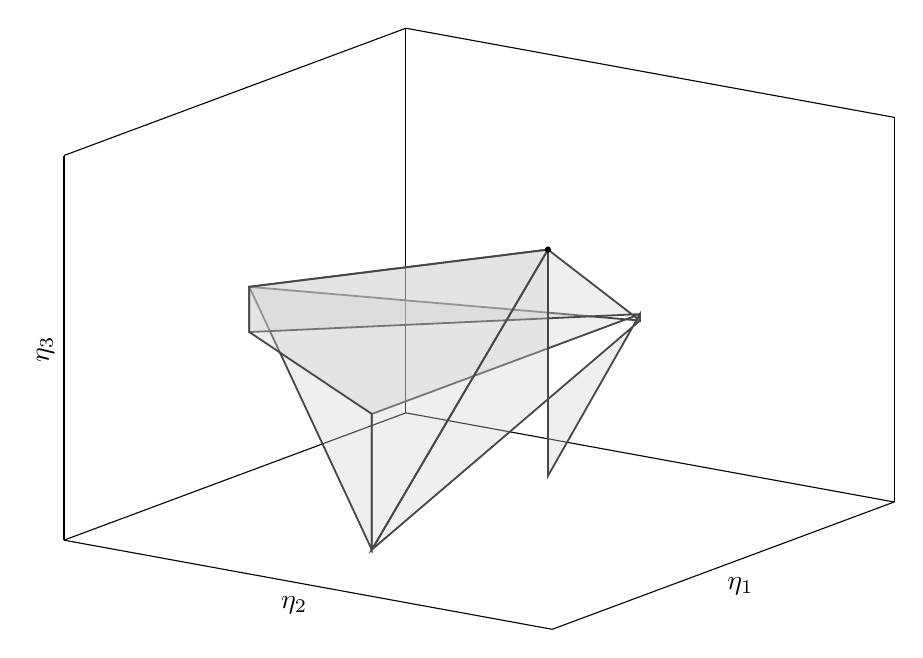
\begin{tikzpicture}
\begin{axis}[
  width=\linewidth,
  height=0.76\linewidth,
  view={125}{22},
  xlabel={\(\eta_1\)},
  ylabel={\(\eta_2\)},
  zlabel={\(\eta_3\)},
  xmin=-0.65,xmax=1.05,
  ymin=-0.65,ymax=1.05,
  zmin=-0.65,zmax=1.05,
  ticks=none,
]
\addplot3[draw=black!72,fill=gray!38,fill opacity=0.34,line width=0.65pt,forget plot] coordinates {
  (-0.6,0.2,-0.0285714285714)
  (0.2,-0.6,0.2)
  (0.733333333333,0.2,-0.6)
} \closedcycle;
\addplot3[draw=black!72,fill=gray!38,fill opacity=0.34,line width=0.65pt,forget plot] coordinates {
  (-0.6,0.2,-0.0285714285714)
  (1,1,1)
  (0.2,-0.6,0.2)
} \closedcycle;
\addplot3[draw=black!72,fill=gray!38,fill opacity=0.34,line width=0.65pt,forget plot] coordinates {
  (-0.6,0.2,-0.0285714285714)
  (0.733333333333,0.2,-0.6)
  (1,1,1)
} \closedcycle;
\addplot3[draw=black!72,fill=gray!38,fill opacity=0.34,line width=0.65pt,forget plot] coordinates {
  (0.2,-0.6,0.2)
  (1,1,1)
  (0.733333333333,0.2,-0.6)
} \closedcycle;

\addplot3[only marks,mark=*,mark size=0.9pt] coordinates {(1,1,1)};
\end{axis}
\end{tikzpicture}

\small (a) all channels
\end{minipage}
\begin{minipage}[t]{0.48\textwidth}
\centering
\begin{tikzpicture}
\begin{axis}[
  width=\linewidth,
  height=0.76\linewidth,
  view={125}{22},
  xlabel={\(\eta_1\)},
  ylabel={\(\eta_2\)},
  zlabel={\(\eta_3\)},
  xmin=0,xmax=1.05,
  ymin=0,ymax=1.05,
  zmin=0,zmax=1.05,
  ticks=none,
]
\addplot3[draw=cbOrange!85!black,fill=cbOrange,fill opacity=0.27,line width=0.65pt,forget plot] coordinates {
  (0,0,0.238095238095)
  (0,0.5,0.357142857143)
  (1,1,1)
  (0.5,0,0.5)
} \closedcycle;
\addplot3[draw=cbOrange!85!black,fill=cbOrange,fill opacity=0.27,line width=0.65pt,forget plot] coordinates {
  (0,0.333333333333,0)
  (0.833333333333,0.5,0)
  (1,1,1)
  (0,0.5,0.357142857143)
} \closedcycle;
\addplot3[draw=cbOrange!85!black,fill=cbOrange,fill opacity=0.27,line width=0.65pt,forget plot] coordinates {
  (0.5,0,0.5)
  (1,1,1)
  (0.833333333333,0.5,0)
  (0.555555555556,0,0)
} \closedcycle;
\addplot3[draw=cbOrange!85!black,fill=cbOrange,fill opacity=0.27,line width=0.65pt,forget plot] coordinates {
  (0,0,0)
  (0,0.333333333333,0)
  (0,0.5,0.357142857143)
  (0,0,0.238095238095)
} \closedcycle;
\addplot3[draw=cbOrange!85!black,fill=cbOrange,fill opacity=0.27,line width=0.65pt,forget plot] coordinates {
  (0,0,0)
  (0,0,0.238095238095)
  (0.5,0,0.5)
  (0.555555555556,0,0)
} \closedcycle;
\addplot3[draw=cbOrange!85!black,fill=cbOrange,fill opacity=0.27,line width=0.65pt,forget plot] coordinates {
  (0,0,0)
  (0.555555555556,0,0)
  (0.833333333333,0.5,0)
  (0,0.333333333333,0)
} \closedcycle;

\addplot3[only marks,mark=*,mark size=0.9pt] coordinates {(1,1,1)};
\end{axis}
\end{tikzpicture}

\small (b) nonnegative spectrum
\end{minipage}
\par\medskip
\begin{minipage}[t]{0.48\textwidth}
\centering
\begin{tikzpicture}
\begin{axis}[
  width=\linewidth,
  height=0.76\linewidth,
  view={125}{22},
  xlabel={\(\eta_1\)},
  ylabel={\(\eta_2\)},
  zlabel={\(\eta_3\)},
  xmin=0,xmax=1.05,
  ymin=0,ymax=1.05,
  zmin=0,zmax=1.05,
  ticks=none,
]
\addplot3[draw=cbOrange!85!black,fill=cbOrange,fill opacity=0.27,line width=0.65pt,forget plot] coordinates {
  (0,0,0.238095238095)
  (0,0.5,0.357142857143)
  (1,1,1)
  (0.5,0,0.5)
} \closedcycle;
\addplot3[draw=cbOrange!85!black,fill=cbOrange,fill opacity=0.27,line width=0.65pt,forget plot] coordinates {
  (0,0.333333333333,0)
  (0.833333333333,0.5,0)
  (1,1,1)
  (0,0.5,0.357142857143)
} \closedcycle;
\addplot3[draw=cbOrange!85!black,fill=cbOrange,fill opacity=0.27,line width=0.65pt,forget plot] coordinates {
  (0.5,0,0.5)
  (1,1,1)
  (0.833333333333,0.5,0)
  (0.555555555556,0,0)
} \closedcycle;
\addplot3[draw=cbOrange!85!black,fill=cbOrange,fill opacity=0.27,line width=0.65pt,forget plot] coordinates {
  (0,0,0)
  (0,0.333333333333,0)
  (0,0.5,0.357142857143)
  (0,0,0.238095238095)
} \closedcycle;
\addplot3[draw=cbOrange!85!black,fill=cbOrange,fill opacity=0.27,line width=0.65pt,forget plot] coordinates {
  (0,0,0)
  (0,0,0.238095238095)
  (0.5,0,0.5)
  (0.555555555556,0,0)
} \closedcycle;
\addplot3[draw=cbOrange!85!black,fill=cbOrange,fill opacity=0.27,line width=0.65pt,forget plot] coordinates {
  (0,0,0)
  (0.555555555556,0,0)
  (0.833333333333,0.5,0)
  (0,0.333333333333,0)
} \closedcycle;

\addplot3[
  surf,
  shader=flat,
  draw=green!35!black,
  line width=0.08pt,
  fill opacity=0.32,
  mesh/rows=33,
] table {generated/spin3_markov_face_1.dat};
\addplot3[
  surf,
  shader=flat,
  draw=green!35!black,
  line width=0.08pt,
  fill opacity=0.32,
  mesh/rows=33,
] table {generated/spin3_markov_face_2.dat};
\addplot3[
  surf,
  shader=flat,
  draw=green!35!black,
  line width=0.08pt,
  fill opacity=0.32,
  mesh/rows=33,
] table {generated/spin3_markov_face_3.dat};
\addplot3[only marks,mark=*,mark size=0.9pt] coordinates {(1,1,1)};
\end{axis}
\end{tikzpicture}

\small (c) embeddable closure within (b)
\end{minipage}
\caption{Spin \(3/2\).  Panels (a) and (b) are generated from exact
rational polytope vertices.  Panel (c) overlays the three green
embeddable-boundary surfaces on the orange nonnegative-spectrum
polytope.  Each surface is obtained by setting one canonical rate to
zero and uses the other rates in \([0,8]\), while the defining cone is
unbounded.}
\label{fig:spin-three-halves-regions}
\end{figure}

\clearpage

\section{Differentiable CP-divisible paths}

\begin{definition}[CP-divisibility]
A family of channels \(\{\Phi_t\}_{t\in I}\) is CP-divisible if for
every \(s\leq t\) in \(I\) there is a channel \(V_{t,s}\) such that
\(\Phi_t=V_{t,s}\Phi_s\).
\end{definition}

\begin{lemma}[Finite-dimensional local criterion]
\label{lem:local-divisibility}
Let \(t\mapsto\Phi_t\) be an invertible \(C^1\) path of channels on a
finite-dimensional matrix algebra.  It is CP-divisible if and only if
\begin{equation}\label{eq:time-local-generator}
 K_t=\dot\Phi_t\Phi_t^{-1}
\end{equation}
is a GKSL generator for every \(t\).
\end{lemma}

\begin{proof}
If the path is CP-divisible, invertibility makes the propagator unique:
\(V_{t+h,t}=\Phi_{t+h}\Phi_t^{-1}\).  It is a channel and
\begin{equation*}
 V_{t+h,t}=\id+hK_t+o(h).
\end{equation*}
The tangent-cone form of the finite-dimensional GKS theorem
\cite[Theorem~2.2 and its conditional-complete-positivity proof]
{GoriniKossakowskiSudarshan1976} says exactly that \(K_t\) is a GKSL
generator.

Conversely, suppose every \(K_t\) is a GKSL generator.  Put
\(\Delta=(t-s)/n\).  The chronological Euler products
\begin{equation*}
 V^{(n)}_{t,s}=
 \exp(\Delta K_{s+(n-1)\Delta})\cdots
 \exp(\Delta K_{s+\Delta})\exp(\Delta K_s)
\end{equation*}
converge in operator norm to the solution of
\(\partial_tV_{t,s}=K_tV_{t,s}\), \(V_{s,s}=\id\).  Indeed, if
\(B=\sup_{u\in[s,t]}\|K_u\|\) and
\begin{equation*}
 \omega_K(\delta)=
 \sup_{\substack{u,v\in[s,t]\\|u-v|\leq\delta}}
 \|K_u-K_v\|,
\end{equation*}
then variation of constants between the exact solution and the
piecewise-constant evolution gives
\begin{equation*}
 \|V_{t,s}-V^{(n)}_{t,s}\|
 \leq (t-s)e^{B(t-s)}\omega_K(\Delta)\longrightarrow0.
\end{equation*}
Every factor is a channel, and the cone of completely positive maps
and the trace-preserving affine subspace are operator-norm closed.
Hence \(V_{t,s}\) is a channel.  Finally, both \(\Phi_t\) and
\(V_{t,s}\Phi_s\) solve \(\dot Y_t=K_tY_t\) with initial value
\(Y_s=\Phi_s\); uniqueness for finite-dimensional linear ODEs gives
\(\Phi_t=V_{t,s}\Phi_s\).
\end{proof}

\begin{theorem}[Instantaneous logarithmic cone]
\label{thm:path-criterion}
Let \(t\mapsto\Phi_t\) be an invertible \(C^1\) path of
\(\SU\)-covariant channels, with tensor-sector eigenvalues
\(\eta_\ell(t)\).  Then the path is CP-divisible if and only if
\begin{equation}\label{eq:path-cone}
 (M^{(j)})^{-1}\frac{d}{dt}
 \begin{pmatrix}
 \log|\eta_1(t)|\\ \vdots\\ \log|\eta_{2j}(t)|
 \end{pmatrix}
 \in\Rplus^{2j}
 \quad\text{for every }t.
\end{equation}
If \(\Phi_{t_0}=\id\) at some \(t_0\), then every
\(\eta_\ell(t)>0\) and the absolute values may be omitted.
\end{theorem}

\begin{proof}
Lemma~\ref{lem:sector-diagonalization} makes every \(\eta_\ell(t)\)
real, while invertibility makes it nonzero.  Since the parameter set is
an interval, continuity makes the sign of each \(\eta_\ell\) constant.
At an identity point all these signs are positive.
Both \(\dot\Phi_t\) and \(\Phi_t^{-1}\) commute with every
\(\cU_g\), so the time-local generator \(K_t\) in
\eqref{eq:time-local-generator} is covariant.  On \(V_\ell\) it acts
by
\begin{equation*}
 \frac{\dot\eta_\ell(t)}{\eta_\ell(t)}
 =\frac{d}{dt}\log|\eta_\ell(t)|.
\end{equation*}
Apply Lemma~\ref{lem:local-divisibility}, then
Theorems~\ref{thm:generator-classification} and
\ref{thm:eigenmatrix}.
\end{proof}

\begin{corollary}[Spin-\(1/2\) negative-spectrum branches]
\label{cor:negative-spectrum-paths}
Let \(t\mapsto\Phi_t\) be an invertible \(C^1\) path of spin-\(1/2\)
covariant channels.  Then it is CP-divisible if and only if
\begin{equation*}
 \frac{d}{dt}\log|\eta_1(t)|\leq0.
\end{equation*}
In particular, the constant path at the nonidentity vertex
\(\eta_1=-1/3\) is invertible and CP-divisible.
\end{corollary}

\begin{proof}
Corollary~\ref{cor:spin-one-half} gives
\((M^{(1/2)})^{-1}=-1/2\), so Theorem~\ref{thm:path-criterion}
reduces to the displayed inequality.  The constant vertex path has
zero logarithmic derivative, and its propagators are the identity
channel.
\end{proof}

\section{Exact computation and reproducibility}

The symbolic calculation has two independent inputs: the Wigner
\(6j\) formula \eqref{eq:M-definition}, and the tensor matrices in
\eqref{eq:tensor-definition}.  This separation makes the phase and
normalization checks observable rather than folding them into a single
table lookup.

\begin{proposition}[Exact reconstruction protocol]
\label{prop:exact-reconstruction}
For \(2j=1,2,3,4\), the repository's exact-cone script performs all of
the following operations in symbolic arithmetic:
\begin{enumerate}
 \item constructs every \(T_q^{(k)}\) once from Clebsch--Gordan
 coefficients and once from the \(3j\) formula
 \eqref{eq:tensor-definition}, and tests entrywise equality;
 \item constructs the matrix of \(\beta\) in
 \eqref{eq:dual-intertwiner}, tests its unitarity, and tests
 \eqref{eq:dual-tensor-phase} for every \(k,q\);
 \item applies every Kraus sum directly to \(T_0^{(\ell)}\), tests that
 its residual after projection onto \(T_0^{(\ell)}\) vanishes, and
 tests that the extracted scalar equals \eqref{eq:M-definition};
 \item tests \eqref{eq:M-from-vertices}, the closed inverse
 \eqref{eq:M-inverse-formula}, and
 \(|\det M^{(j)}|=2j+1\).
\end{enumerate}
The primitive integer rows printed by the script are exactly the facet
normals in the spin-\(1\), spin-\(3/2\), and spin-\(2\) corollaries.
\end{proposition}

\begin{proof}
The tensor and Wigner routines return SymPy algebraic numbers, and the
tests use exact matrix equality after symbolic simplification.  The
direct Kraus reconstruction does not call the \(6j\)-based generator
routine.  For each \((\ell,k)\), it first checks the matrix identity
\(\cD_k(T_0^{(\ell)})=m_{\ell k}T_0^{(\ell)}\), including the full
residual, and then compares \(m_{\ell k}\) with
\eqref{eq:M-definition}.  Thus items 1--3 compare the two derivations
entry by entry; item 4 substitutes the resulting matrices into the
displayed algebraic identities.  The executable check is
\begin{equation*}
 \texttt{python3 -u code/exact\_cones.py 1 2 3 4 --verify}.
\end{equation*}
\end{proof}

\begin{proposition}[Exact polytope certificates]
\label{prop:exact-polytope-certificates}
The script \texttt{code/generate\_plot\_data.py} enumerates every
full-rank active set of the spin-\(1\) and spin-\(3/2\) simplex
halfspaces together with \(\eta_\ell\geq0\), solves the systems over
the rationals, and records each feasible vertex, its barycentric
coordinates, the exact polytope volumes, and the embeddable-region
Jacobian volumes in \texttt{paper/generated/geometry\_exact.txt}.
The only floating-point data produced by the script are plotting
coordinates: the spin-\(1\) curves and the truncated spin-\(3/2\)
boundary meshes.
\end{proposition}

\begin{proof}
There are finitely many choices of as many active inequalities as the
ambient dimension.  A polytope vertex occurs in at least one full-rank
choice.  The script iterates over all choices, discards singular systems,
solves the rest over \(\mathbb Q\), and retains exactly the points that
satisfy every halfspace.  It then computes barycentric coordinates by
the inverse augmented vertex matrix.  Boundary cycles are ordered by
exact signs of rational planar cross products.  The certificate records
those cycles and every rational determinant term in the shoelace and
pyramid sums, so no floating-point decision enters a stated area or
volume.  This is the active-set argument used in
Proposition~\ref{prop:comparison-polytopes}.
\end{proof}

From the repository root, \texttt{make check} runs the exact tensor
audit, \texttt{make figures} regenerates all plot data and certificates,
and \texttt{make paper} rebuilds the figures, bibliography, and paper.

\section{Conclusion}

For a fixed irreducible spin, covariance converts the canonical GKS
matrix into one nonnegative rate per nonzero tensor rank.  Recoupling
then converts those rates to sector decay exponents by the matrix
\(M^{(j)}\), while orthogonality of the Racah transform supplies the
closed inverse \eqref{eq:M-inverse-formula}.  Endpoint embedding is
therefore a finite set of linear inequalities in logarithmic
eigenvalues, and time-dependent CP-divisibility is the pointwise version
of the same test applied to logarithms of absolute sector eigenvalues.
The low-spin corollaries and comparison plots make
the distinction between complete positivity, positive spectrum, and
covariant Markovian embeddability explicit.

\bibliographystyle{plain}
\bibliography{references}

\end{document}
